\documentclass[11pt, oneside]{article} 
\usepackage{geometry}
\geometry{letterpaper} 
\usepackage{graphicx}
	
\usepackage{amssymb}
\usepackage{amsmath}
\usepackage{parskip}
\usepackage{color}
\usepackage{hyperref}

\graphicspath{{/Users/telliott_admin/Dropbox/Tex/png/}}
% \begin{center} 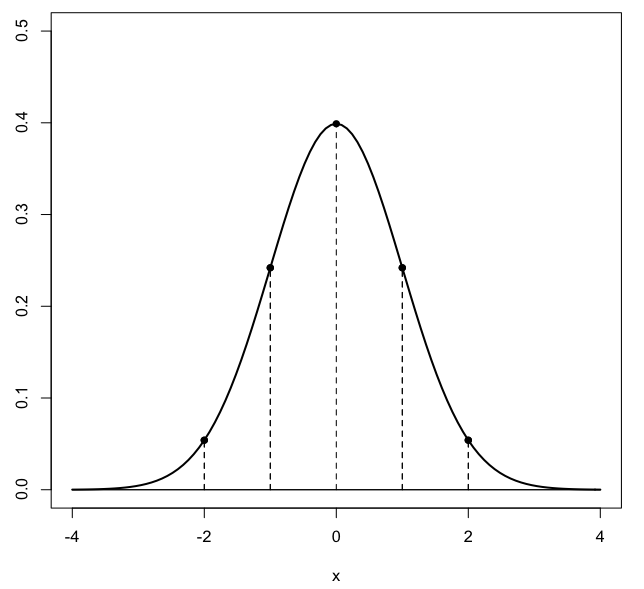
\includegraphics [scale=0.4] {gauss3.png} \end{center}

%break
\title{Double and half angles}
\date{}

\begin{document}
\maketitle
\Large

\label{sec:double_half_angles}

We will find it useful in several problems to be able to compute the sine, cosine and tangent of angle $2\theta$, knowing the values for $\theta$.  These formulas can be rearranged to give the values of $\theta/2$ in terms of $\theta$.

I can't remember these formulas, but derive them from the sum of angles when needed.

\subsection*{cosine}

Start with our old friend:

\[ \cos s + t = \cos s \cos t - \sin s \sin t \]

Let $s=t$:
\[ \cos 2s = \cos^2 s - \sin^2 s \]
Since $\sin^2 s + \cos^2 s = 1$, $-\sin^2 = \cos^2 - 1$ so
\[  \cos 2s = 2 \cos^2 s - 1 \]

We can use this formula to compute the value for $2s$ given that for $s$.  To go from $2\theta$ to $\theta$:
\[ \cos^2 s = \frac{1}{2}(1 + \cos 2s) \]
\[ \cos s = \sqrt{ \frac{1}{2}(1 + \cos 2s)} \]

\subsection*{sine}
\[ \sin s + t = \sin s \cos t + \cos t \sin s \]

Let $s = t$:
\[ \sin 2s = 2 \sin s \cos s \]

Put the other way
\[ \sin s = \frac{\sin 2s}{2 \cos s} \]

\subsection*{tangent}

The formulas for the tangent are easily obtained by substitution.  Let us simplify the notation a bit by setting $S = \sin 2t$ and $S' = \sin t$ and similarly for cosine and tangent.  From above we have the basic relationships

\[ S' = \frac{S}{2 C'} \]
and
\[ C' = \sqrt{\frac{1}{2} (1 + C)}  \]
\[ 2[C']^2 = 1 + C \]

So the tangent ($T' = \tan s$) is:
\[ T' = \frac{S'}{C'} = \frac{S}{2C'} \ \frac{1}{C'} = \frac{S}{2 [C']^2} \]
\[ = \frac{S}{1 + C} \]
That's a fairly remarkable simplification!

Another way to say the same thing:
\[ \frac{1}{T'} = \frac{1}{T} + \frac{1}{S} \]

This result can be massaged in various ways.  Multiply on the top and bottom of the right-hand side by $T$
\[ T' = \frac{ST}{S + T} \]

Also, since
\[ T'  = \frac{S}{1 + C} = \frac{S'}{C'} \]
\[ C' = \frac{S'(1+C)}{S} \]

In going from unprimed ($2 \theta$) to prime ($\theta$), it seems that the most straightforward way is to compute

\[ C' = \sqrt{\frac{1}{2} (1 + C)}  \]
\[ T'  = \frac{S}{1 + C} \]
and then the sine last
\[ S' = \frac{S}{2 C'} \]

\subsection*{check}

Let's try checking the results for a known angle
\[ 2 \theta = \pi/3 \]
\[ S = \sin 2 \theta = \frac{\sqrt{3}}{2}, \ \ \ \cos 2 \theta = \frac{1}{2}, \ \ \ T = \tan 2 \theta = \sqrt{3} \]
\[ S' = \sin \theta = \frac{1}{2}, \ \ \ \cos \theta = \frac{\sqrt{3}}{2}, \ \ \ T' = \tan \theta = \frac{1}{\sqrt{3}} \]
Our first equation is
\[ T' =  \frac{ST}{S+T} = \frac{3/2}{(3/2)\sqrt{3}} = \frac{1}{\sqrt{3}} \]

That looks good.  The second one is
\[ S' = \sqrt{\frac{ST'}{2}} \]
\[ ST' = \frac{\sqrt{3}}{2} \frac{1}{\sqrt{3}} = \frac{1}{2} \]
\[ S' = \sqrt{ \frac{1}{2}\ \ \frac{1}{2}} = \frac{1}{2} \]
These both look correct.

\subsection*{geometric approach}

Here are two simple geometric derivations of the half angle formulas for sine and cosine.

\begin{center} 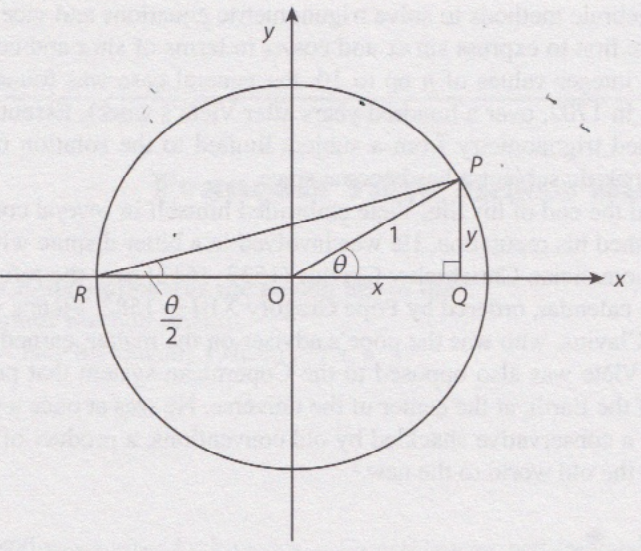
\includegraphics [scale=0.4] {half_angle_simple.png} \end{center}
For the first, draw an angle $\theta$ in a unit circle.  We proved the theorem that the angle at the left (on the circle) is equal to $\theta/2$ \hyperref[sec:generalized_arc]{\textbf{here}}.

Algebraically, write
\[ \cos \frac{\theta}{2} = \frac{1 + x}{\sqrt{(1 + x)^2 + y^2}} \]
\[ = \frac{1 + x}{\sqrt{1 + 2x + x^2 + y^2}} \]
\[ = \frac{1 + x}{\sqrt{2 + 2x}} \]
\[ = \sqrt{\frac{1 + \cos \theta}{2}} \]
To get the formula for the sine just use the identity
\[ \cos^2  \frac{\theta}{2} + \sin^2  \frac{\theta}{2} = 1 \]
\[ \sin^2  \frac{\theta}{2} = 1 - \frac{1 + \cos \theta}{2}  = \frac{1 - \cos \theta}{2} \]
Using the prime notation from above
\[ S' = \sqrt{\frac{1 - C}{2}} \]
This is easily checked
\[ S'^2 + C'^2 = 1 \]
\[ \frac{1 - C}{2} + \frac{1 +C}{2} = 1 \]
which looks correct.

For the second derivation, again draw an angle $\theta$ in a unit circle.  As usual, then, the base of the right triangle is $\cos \theta$ and the height is $\sin \theta$ (left panel, below).

Now, also draw the chord of the circle, corresponding to the arc $\theta$.

\begin{center} 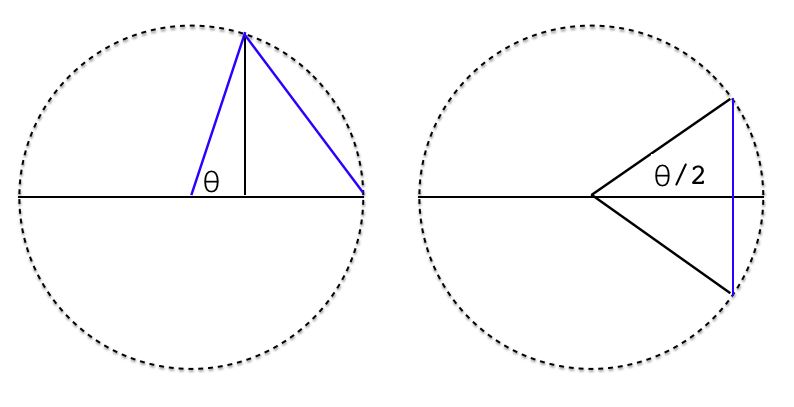
\includegraphics [scale=0.4] {half_angle.png} \end{center}
Notice that the chord is the hypotenuse of a right triangle whose height is $\sin \theta$ and whose base is $1 - \cos \theta$.  Therefore, the length of the chord is
\[ c = \sqrt{(1 - \cos \theta)^2 + \sin^2 \theta} = \sqrt{2 - 2 \cos \theta} \]
Now, rotate the chord as shown in the right panel.  We see that one-half the chord is equal to the sine of $\theta/2$:
\[ \sin \theta / 2 = \frac{1}{2} \ \sqrt{2 - 2 \cos \theta} \]
\[ S' = \frac{1}{\sqrt{2}} \ \sqrt{1 - C} \]
and
\[ S'^2 + C'^2 = 1 \]
\[ C'2 = 1 - S'^2 = 1 - \frac{1 - C}{2} = \frac{1 + C}{2}  \]
\[ C' = \frac{1}{\sqrt{2}} \ \sqrt{1 + C} \]

\end{document}